\documentclass[12pt,a4paper]{article}
\usepackage{graphicx}
\usepackage[utf8]{inputenc}
\usepackage{hyperref}
\usepackage{pgfplots}
\usepackage{mathtools}

\begin{document}
\begin{titlepage}
	\centering
	
\includegraphics[width=0.15\textwidth]{utec.png}\par\vspace{1cm}
	{\scshape\LARGE UTEC \par}
	\vspace{1cm}
	{\scshape\Large Procesador MIPS 32\par}
	\vspace{1.5cm}
	{\huge\bfseries Arquitectura de las Computadoras\par}
	\vspace{2cm}
	{\Large\itshape Alejandro Goicochea\par}
	\href{mailto:alejandro.goicochea@utec.edu.pe}{alejandro.goicochea@utec.edu.pe}
	\vfill
	Profesor:\par
	Jorge Gonzales

	\vfill
	{\large \today\par}
\end{titlepage}

\section{Introducción}
En este reporte se va a documentar la implementación de un procesador MIPS32 en verilog. Para las instrucciones se implementaran algunas instrucciones del instruction set detallado en el MIPS reference data card del siguiente enlace:
\href{https://inst.eecs.berkeley.edu/~cs61c/resources/MIPS_Green_Sheet.pdf}{MIPS Resource Data Sheet}\\
Las instrucciones implementadas son las siguientes:\\

\begin{table}[htb]
\begin{center}
\begin{tabular}{|l|l|l|l|}
\hline
add & addi & lb  & beq  \\ \hline
sub & andi & lh  & bneq \\ \hline
and & ori  & lw  & bgez \\ \hline
nor & slti & sb  & j    \\ \hline
or  &      & sh  & jr   \\ \hline
slt &      & sw  & jal  \\ \hline
    &      & lui &      \\ \hline
\end{tabular}
\end{center}
\end{table}

Para el caso de bgez se usara el opcode $000001$.


\section{Implementación}
Para la implementación del procesador se usaron los siguientes módulos:
\begin{enumerate}
\item DataPath
\item InstructionMemory
\item InstructionProcess
\item Registers
\item DataMemory
\item ALU
\item ControlUnit
\item MemToReg
\end{enumerate}

\subsection{Datapath}
\text Este módulo es la base del procesador, se encarga de enviar la información a todos los otros módulos mediante wires y de la declaración de todos los registros que se van a usar como las señales y registros. Además, se encarga de los incrementos del $PC$ a través de los jumps y branches o un incremento de 4.

\subsection{InstructionMemory}
\text En este módulo se almacenan las instrucciones en un registro desde un archivo de texto y se devuelve una instrucción cada vez
que llega un $PC$. Las instrucciones se guardan en bytes por lo que el módulo concatena 4 direcciones para devolver la instrucción completa.

\subsection{InstructionProcess}
\text En este módulo se divide la instrucción en sus diferentes partes dependiendo del tipo de instrucción. Toma siempre el opcode ya que los primeros 6 bits siempre le van a pertenecer y con eso sabe cómo partir el resto de los bits.

\subsection{Registers}
\text Este módulo se encarga de los 32 registros con los que cuenta el procesador. Está separado en dos bloques $always$ uno para escritura y otro para lectura por lo que tiene dos señales que habilitan estos bloques. Para el bloque de escritura, también se cuenta con una señal para ver si se escribe a la dirección de rd o rt dependiendo si es una instrucción de tipo $R$ o $I$. En caso sea una instrucción de tipo $I$ se revisa el opcode en caso de que sea una instrucción load que tiene diferente comportamiento a las demás. Los registros están cargados inicialmente con puros $0$ de un archivo de texto.

\subsection{DataMemory}
\text En el DataMemory se maneja el caché del procesador. Esta se carga de un archivo de texto lleno de 0. Cuenta con dos funciones, escritura y lectura. El módulo solo se llama para las instrucciones de load y store, mandando datos al registro en caso de loads y almacenando en la memoria en caso de store. Cuenta también con dos señales: $memWrite$ y $memRead$ para determinar la operación que se hace.

\subsection{ALU}
\text La ALU se encarga de todas las operaciones aritméticas de nuestras instrucciones. También se encarga de determinar si se toma un branch o no. Siempre se revisa el opcode primero para ver si la instrucción es de tipo $R$ por lo que se pasa a revisar el valor de $funct$. La ALU también crea registros de tipo signed para las operaciones de suma o resta, calcula la dirección del branch, y la dirección de los stores y loads.

\subsection{MemToReg}
\text El módulo MemToReg es un multiplexer de 2 a 1 que se encarga de seleccionar que se va a mandar al módulo de registros para escritura. El selector de este multiplexer depende del tipo de instrucción que se está ejecutando.

\section{Diagrama}

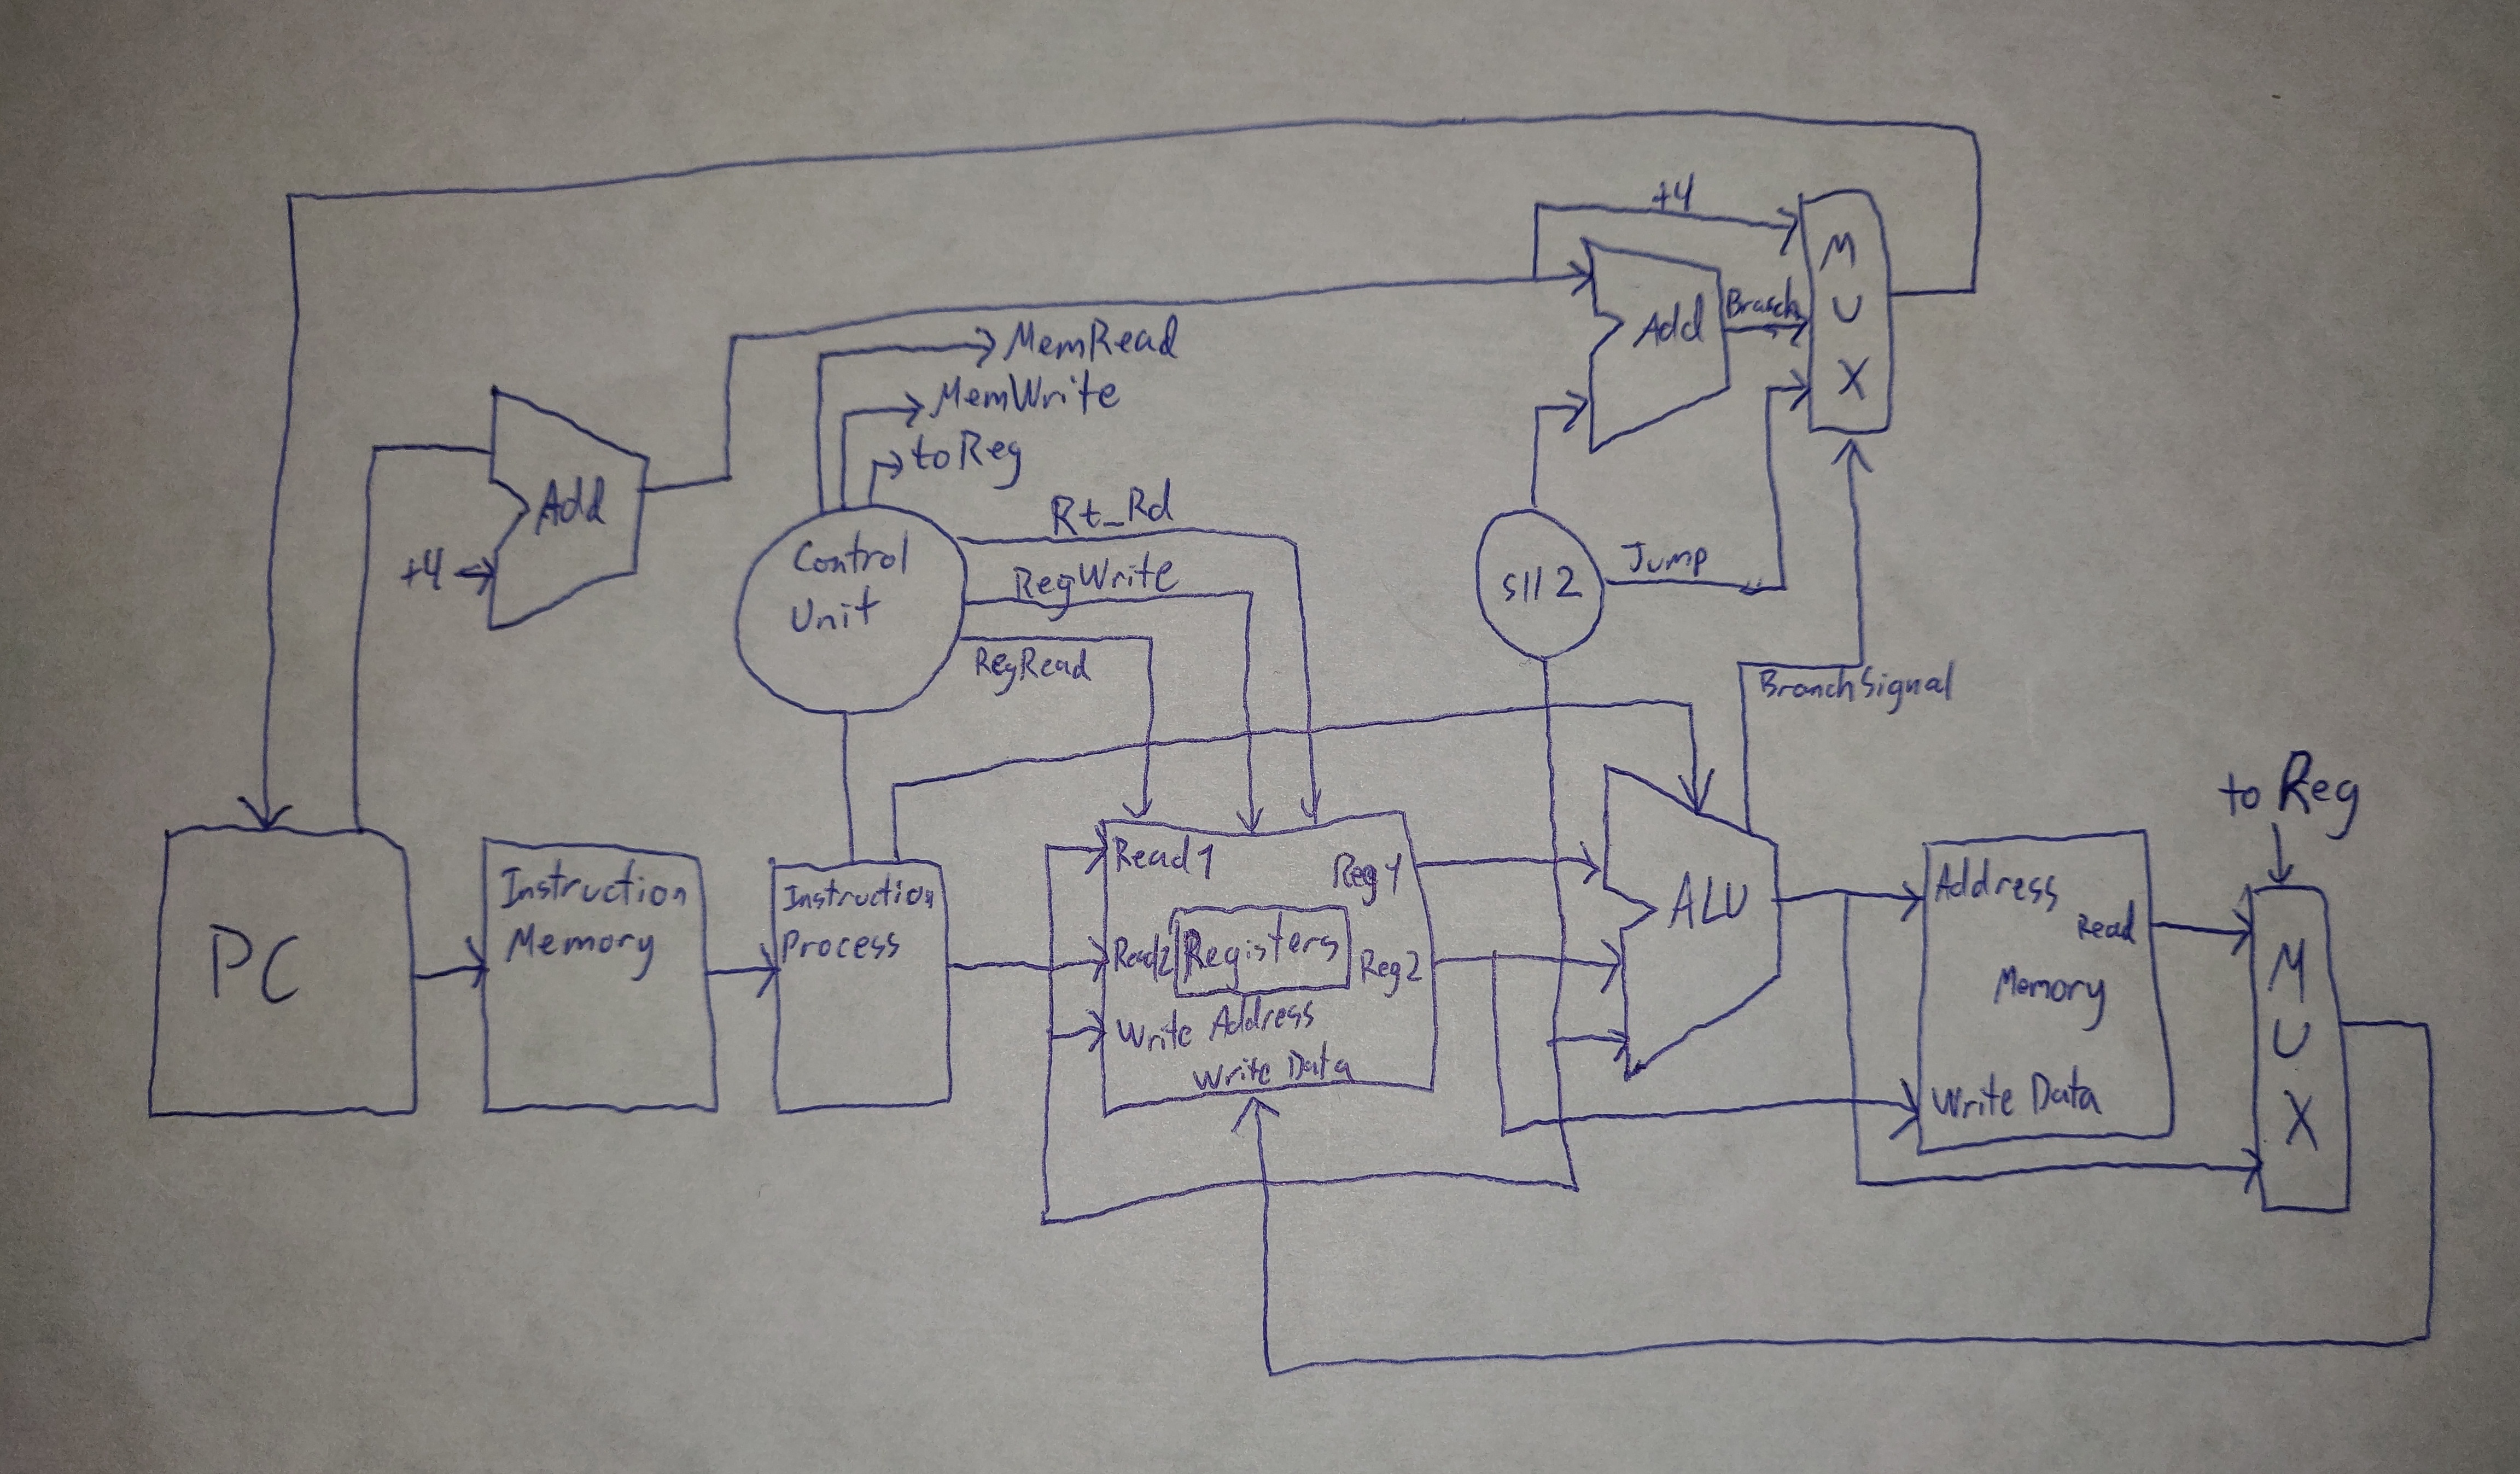
\includegraphics[width=14cm]{./datapath.jpg}

\newpage

\section{Conclusiones}
El procesador puede ejecutar todas las instrucciones propuestas exitosamente. Se crearon 3 programas para ejecutarlas. El primero ejecuta las dos primeras columnas de las instrucciones detalladas en la sección 1, el segundo la tercera columna y el tercer programa la cuarta columna. Para el debugging del procesador se usó el comando $display$ en varios lugares los cuales terminaron siendo usados para comprobar que el datapath funcione correctamente. Cada módulo ejecuta un $display$ dependiendo de las operaciones que ejecute las cuales detallan la ejecución de cada programa. El procesador implementado, aunque funcione correctamente, utiliza más hardware que un procesador común y gracias a las facilidades que ofrece el lenguaje usado se implementan algunos MUX dentro de los módulos  para reducir la cantidad de wires y módulos usados simplificando su lectura y comprensión.



\end{document}
